\documentclass[varwidth=true, border=2pt]{standalone}

\usepackage{pgfplots}
\usepackage{tikz}

\begin{document}
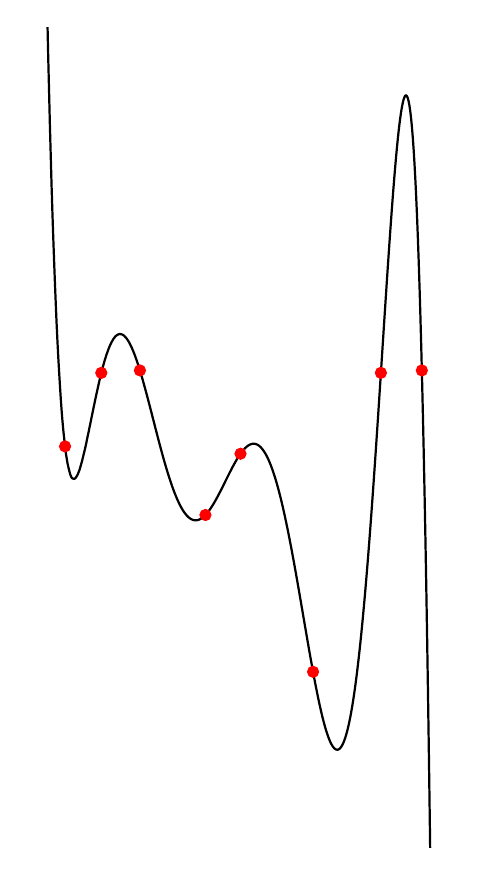
\begin{tikzpicture}
    \begin{axis}[
        %legend pos=south east,
        axis x line=none,
        axis y line=none,
        %grid = major,
        width=8cm,
        height=12cm,
        %grid style={dashed, gray!30},
        xmin=-90,     % start the diagram at this x-coordinate
        xmax= 30,    % end   the diagram at this x-coordinate
        ymin=-36,     % start the diagram at this y-coordinate
        ymax= 57,   % end   the diagram at this y-coordinate
        %axis background/.style={fill=white},
        xlabel=x,
        ylabel=y,
        %xticklabels={-2,-1.6,...,2},
        %yticklabels={-8,-7,...,8},
        %tick align=outside,
        enlargelimits=true,
        tension=0.08]
        \addplot[domain=-90:30, black, thick,samples=500] {-30.550224302876202 +1.3405464324655687*x +0.33940746902954505*x*x +0.006043447628845429*x*x*x -0.00040762779516188906*x*x*x*x -0.000016598804950050045*x*x*x*x*x -2.1597800840011248e-7*x*x*x*x*x*x +-9.533599505095986e-10*x*x*x*x*x*x*x}; 
      %\addplot[domain=-90:30, red, thick,samples=500] {-107/168000000*x^5 -5053/50400000*x^4 -103/28800*x^3	+1237/20160*x^2	+59573/25200*x	+-77/15}; 
        \addplot[red, only marks, mark=*] coordinates {(-79.66666666666667,9.333333333333329) (-69.33333333333333,19.33333333333333) (-58.333333333333336, 19.66666666666667) (-39.666666666666664,0) (-29.666666666666664,8.333333333333329) (-9,-21.33333333333333) (10.333333333333329,19.33333333333333) (22,19.66666666666667)};
      %\addlegendentry{$f(x)=x^3$}
    \end{axis} 
\end{tikzpicture}
\end{document}
